%!TEX root = ../../architekturdokumentation.tex
\chapter{Logische Architektur}
\subsection{3-Tier-Architektur}
		Um eine möglichst hohe Abstraktion unseres Codes zu erhalten, haben wir uns für eine 3-Tier-Architektur entschieden, die unsere Applikation in die drei Schichten Web, Service und DataAccesLayer (Dal) unterteilt. Alle Datenbankspezifischen Operationen sollen im DAL vorgenommen werden. Alle Zugriffe aus dem Web sollen über die Web-Layer behandelt werden. Die Zugriffe auf externe Schnittstellen über den Service-Layer.
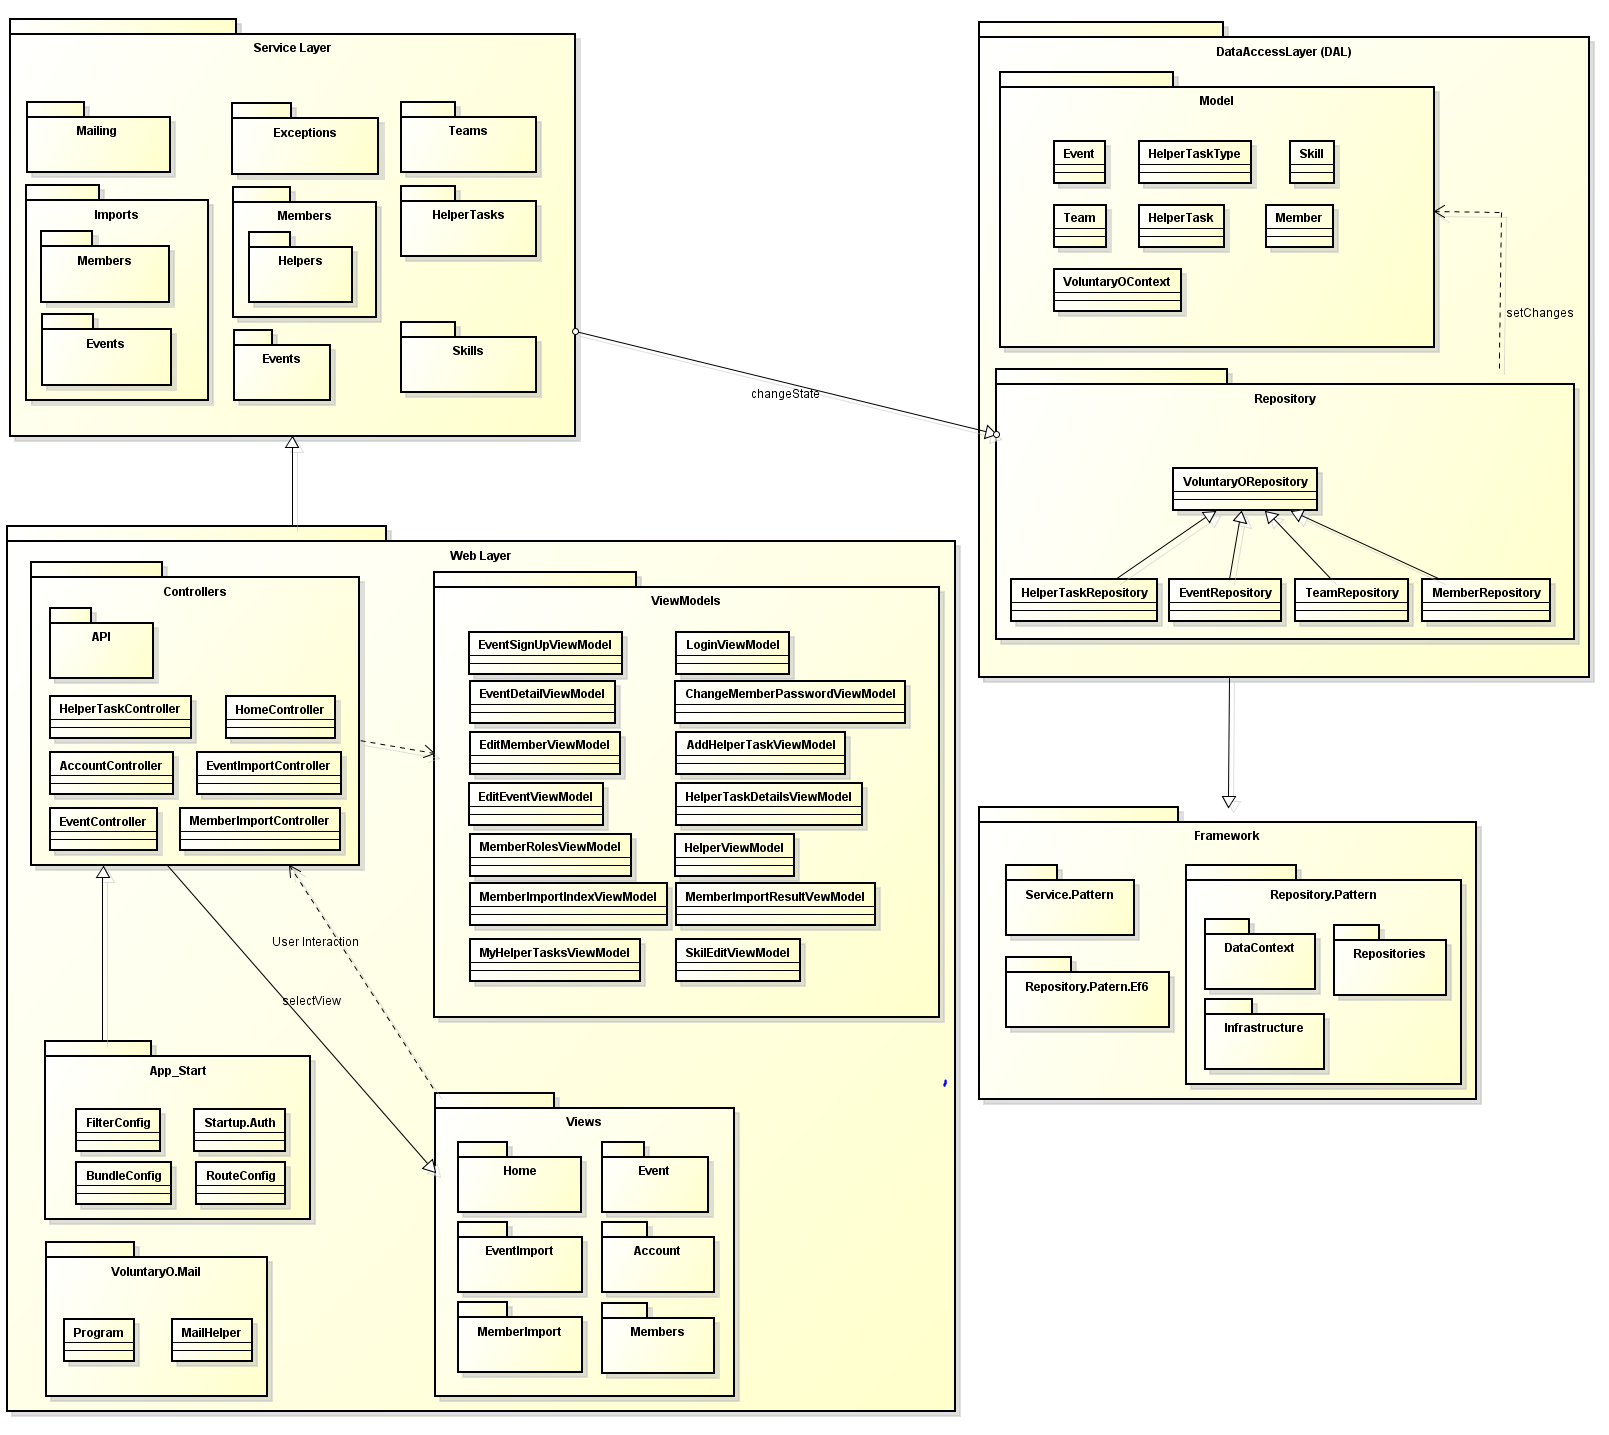
\includegraphics[width=\textwidth]{content/architekturdokumentation/images/LogischeArchitektur.png}
